% Add "answers" option to print the answers
\documentclass[addpoints]{exam}

\usepackage[utf8]{inputenc}
\usepackage{calc}
\usepackage[dvipsnames]{xcolor}
\usepackage{ifthen}
\usepackage{tcolorbox}

% \makebox[\textwidth]{Name:\enspace\hrulefill}
%  
% \vspace{5mm}
%\makebox[\textwidth]{Instructor’s name:\enspace\hrulefill}

\definecolor{MyLightGray}{gray}{0.60}

\newcommand{\truefalse}
{		\begin{checkboxes}
			 \choice True
			 \choice False. Explanation: 
		\end{checkboxes}
		\vspace{10pt}
}


% Check if 'answers' is an option
\newcommand{\ifanswers}[2]{%
  \ifthenelse{\boolean{exam@answers}}{#1}{#2}%
}



\newcommand{\answerspace}[1]
{
	\ifprintanswers
	\else
		\setlength{\mylength}{10pt}%
		% \vspace{#1\mylength}
		% Make the grey box
		\par\nobreak\noindent
		\makebox[\linewidth][l]{%
			% set inner padding to zero, so only the frame shows
			{\setlength{\fboxsep}{0pt}%
			% draw a color frame, white (or transparent) inside
			\fcolorbox{MyLightGray}{white}{%
			% the inner box has zero width content but fixed height
			\parbox[t][#1\mylength][c]{%
				% subtract twice the frame‐thickness from the full width
				\dimexpr\linewidth-2\fboxrule\relax
			}{\strut}%
			}%
			}%
		}%
		\par
		\vspace{3\mylength}

  	\fi
}
\newlength{\mylength}

\newcommand{\code}[1]{{\texttt{#1}}}

\newcommand{\answer}[1]{\begin{solution}{#1}\end{solution}}




%\usepackage{listings}
\usepackage{color}
\usepackage{lastpage}
\usepackage{verbatim}
\usepackage{fancyvrb}
\usepackage{graphicx}
\usepackage{float}
\usepackage{minted}

\newcommand{\includecode}[2][c]{\lstinputlisting[caption=, escapechar=, language=#1]{#2}}
\RecustomVerbatimCommand{\VerbatimInput}{VerbatimInput}{}

\newcommand{\Code}[1]{\mintinline{python}{#1}}
\newcommand{\ACC}[3]{\Code{foo(#1, #2, #3)}}

\renewcommand{\solutiontitle}{\noindent\textbf{Solution sketch: }}

\definecolor{SolutionColor}{rgb}{0.8,0.9,1}

\cfoot{Page \thepage\ of \pageref{LastPage}}

\rhead{Initials: \rule{20mm}{0.4pt}}

\begin{document}
\fvset{numbers=left,numbersep=3pt}
\thispagestyle{empty}

\begin{center}
	{\LARGE CS 408 Fall 2026 -- Midterm 1 (A)\\}

\fbox{\fbox{\parbox{5.5in}{\centering
	\begin{itemize}
        \item The exam is closed notes, closed book.

        \item The exam should be completed individually: any
          communication with your fellow students is \textbf{strictly}
          prohibited.

        \item If you have a question, raise your hand and the
          course staff will come to you.

        \item Please print or write legibly.

        \item Try to be concise: when a question asks for an
          explanation, a few sentences should suffice. Aim for
          quality, not quantity!

        \item Show enough of your reasoning so that we can award
          partial credit for a correct approach.

        \item Answer the questions in the spaces provided. Your answer
          does not need to take up all the space provided (hopefully
          we've given you more than enough room!). If you do run out
          of space, make a note and then use the empty pages at the
          back of the exam to complete your answer. Be sure to clearly
          label any answers on those pages with the corresponding
          question.

        \item Several questions ask you to provide something ``if
          possible.'' If it is not possible, you should plainly say so
          and then explain why that is the case.

        \item Coding questions should be answered in Python, unless
          stated otherwise.

        \item Unless otherwise noted, CFG nodes represent basic
          blocks. When necessary, refer to nodes using the labels
          given in the figure.

        \item Please double check that your copy of the exam
          is complete; you should have \pageref{LastPage}
          pages.

        \item You have 75 minutes to complete the exam.
        \end{itemize}
	}}}
\end{center}

\begin{center}
	\makebox[0.6\textwidth]{
		\combinedgradetable[h][questions]
	}
\end{center}
\vspace{20mm}

\makebox[\textwidth]{\textbf{Name (please print)}: \rule{100mm}{0.8pt} }

\vspace{10mm}
\makebox[\textwidth]{\textbf{PUID}: \rule{40mm}{0.8pt} \hspace{35mm}}

\vspace{10mm}
\makebox[\textwidth]{\textbf{Ticket \#}: \rule{40mm}{0.8pt} \hspace{35mm}}

\newpage
\begin{center}
  [PAGE DELIBERATELY LEFT BLANK]
\end{center}

\begin{questions}

  \newpage

% ========================================================
% Q1: warm-up.  [from final.tex Q1-Q4]
% ========================================================

\question Short answers.
\begin{parts}

\part[1] Under the RIPR model, is it ever possible for a test case to
  trigger an error state without inducing a failure? You may answer
  this question with a simple ``yes'' or ``no''. %
  \answerspace{5} %
  \begin{solution}
    Yes.
  \end{solution}

\part[1] Under the RIPR model, if the program under test does not
  contain a fault, can a test case ever induce a failure? Again, an
  answer of ``yes'' or ``no'' will suffice. %
  \answerspace{5} %
  \begin{solution}
    No.
  \end{solution}

\part[2] Order the following CFG-based coverage criteria using the
  subsumption relation: (A) edge coverage, (B) complete path coverage,
  (C) node coverage, (D) edge-pair coverage. Your answer should have
  the form C $\subseteq$ A $\subseteq$ \ldots, where C is subsumed by
  A, and so on. %
  \answerspace{8} %
  \begin{solution}
    C $\subseteq$ A $\subseteq$ D $\subseteq$ B.
    Node $\subseteq$ edge $\subseteq$ edge-pair $\subseteq$ path.
  \end{solution}

\part[3] For an arbitrary program, is it always possible to find a test
  set that achieves 100\% node coverage for that program? If your
  answer is ``yes'', explain why in 2--3 sentences. If your answer is
  ``no'', provide a short ($\leq$ 5 line) program for which 100\% node
  coverage is impossible. %
  \answerspace{15} %
  \begin{solution}
    No. Test requirements are derived syntactically, but whether a
    node is reachable is a semantic question, and some nodes are
    unreachable. For example:
\begin{minted}{python}
def f(x):
  if x > 0 and x < 0:
    print("unreachable")
\end{minted}
  \end{solution}

\end{parts}

\newpage
\begin{center}
  [PAGE DELIBERATELY LEFT BLANK]
\end{center}
\newpage

% ========================================================
% Q2: black-box vs white-box.  [from midterm.tex Q7+Q8]
% ========================================================

\question Black-box and white-box testing.
\begin{parts}

\part[2] In 1--2 sentences, explain the key difference between
  black-box and white-box testing approaches. %
  \answerspace{18} %
  \begin{solution}
    White-box approaches assume access to the source code of the
    program under test, while black-box approaches assume you can only
    run the program and observe its inputs and outputs.
  \end{solution}

\part[2] Provide one example of a white-box testing technique and one
  example of a black-box testing technique that we have discussed in
  class. %
  \answerspace{18} %
  \begin{solution}
    Black-box: input space partitioning. White-box: any of the
    CFG-based coverage criteria, data-flow coverage, logic coverage,
    or mutation testing.
  \end{solution}

\end{parts}

% ========================================================
% Q3: input space partitioning.  [from midterm.tex Q6]
% ========================================================

\newpage

\question Consider the following Python program:
  \begin{minted}{python}
def calculate_curve(cat: str, grade: float) -> float:
   """ cat is one of "grad", "honors", or "undergrad",
       and grade is a score between 0 and 100. Returns the curved
       grade; graduate students get no curve, honors
       students get a slight curve, and everyone else gets a
       larger curve."""
   ...
\end{minted}
and the following set of blocks:
\begin{center}
\begin{tabular}{c|c|c}
  \textbf{block} & \textbf{Student Status} & \textbf{Original Grade} \\
  \hline
  B$_1$ & \Code{cat == "grad"} & \Code{grade <= 59} (F)\\
  B$_2$ & \Code{cat == "grad"} & \Code{grade < 70} (below C) \\
  B$_3$ & \Code{cat == "honors"} & \Code{grade < 90} (below A)\\
  B$_4$ & \Code{cat == "undergrad"} & \Code{True} (Any grade) \\
\end{tabular}
\end{center}

\begin{parts}
\part[4] Is this a valid partitioning of the input space of
  \Code{calculate_curve}? Explain your answer. %
  \answerspace{15} %
  \begin{solution}
    No. A partition must be \textbf{disjoint} and \textbf{complete},
    and this set of blocks fails both.

    \emph{Disjointness} fails: B$_1$ and B$_2$ overlap, so a graduate
    with a grade of 50 belongs to both.

    \emph{Completeness} fails: many inputs belong to no block at all,
    e.g.\ a graduate with a grade of 85, or an honors student with a
    grade of 95.
  \end{solution}

\part[4] If your answer was ``yes'', provide a set of test cases based
  on this partitioning. If your answer was ``no'', how would you
  modify and/or augment this set of blocks to turn it into a valid
  partitioning?  %
  \answerspace{15} %
  \begin{solution}
    Many correct answers; the requirement is that every input falls in
    exactly one block. One approach is to partition on the two
    characteristics independently and do pairwise testing (i.e.,
    take their cross product): \emph{status} $\in$ \{graduate, honors,
    undergrad\} and \emph{grade} $\in$ \{$< 60$, $60$--$69$,
    $70$--$89$, $\ge 90$\}, giving 12 blocks.

    Full credit for any answer that repairs both properties and says
    which property each change fixes.
  \end{solution}
\end{parts}

\newpage
\begin{center}
  [PAGE DELIBERATELY LEFT BLANK]
\end{center}
\newpage

% Dropping to keep exam length manageable
% ========================================================
% Q4: CFG paths.  [from midterm.tex Q1, part (e) dropped]
% ========================================================

% \question Consider the following control-flow graph:
%   \begin{figure}[ht]
%     \vspace{-.3cm}
%     \begin{center}
%       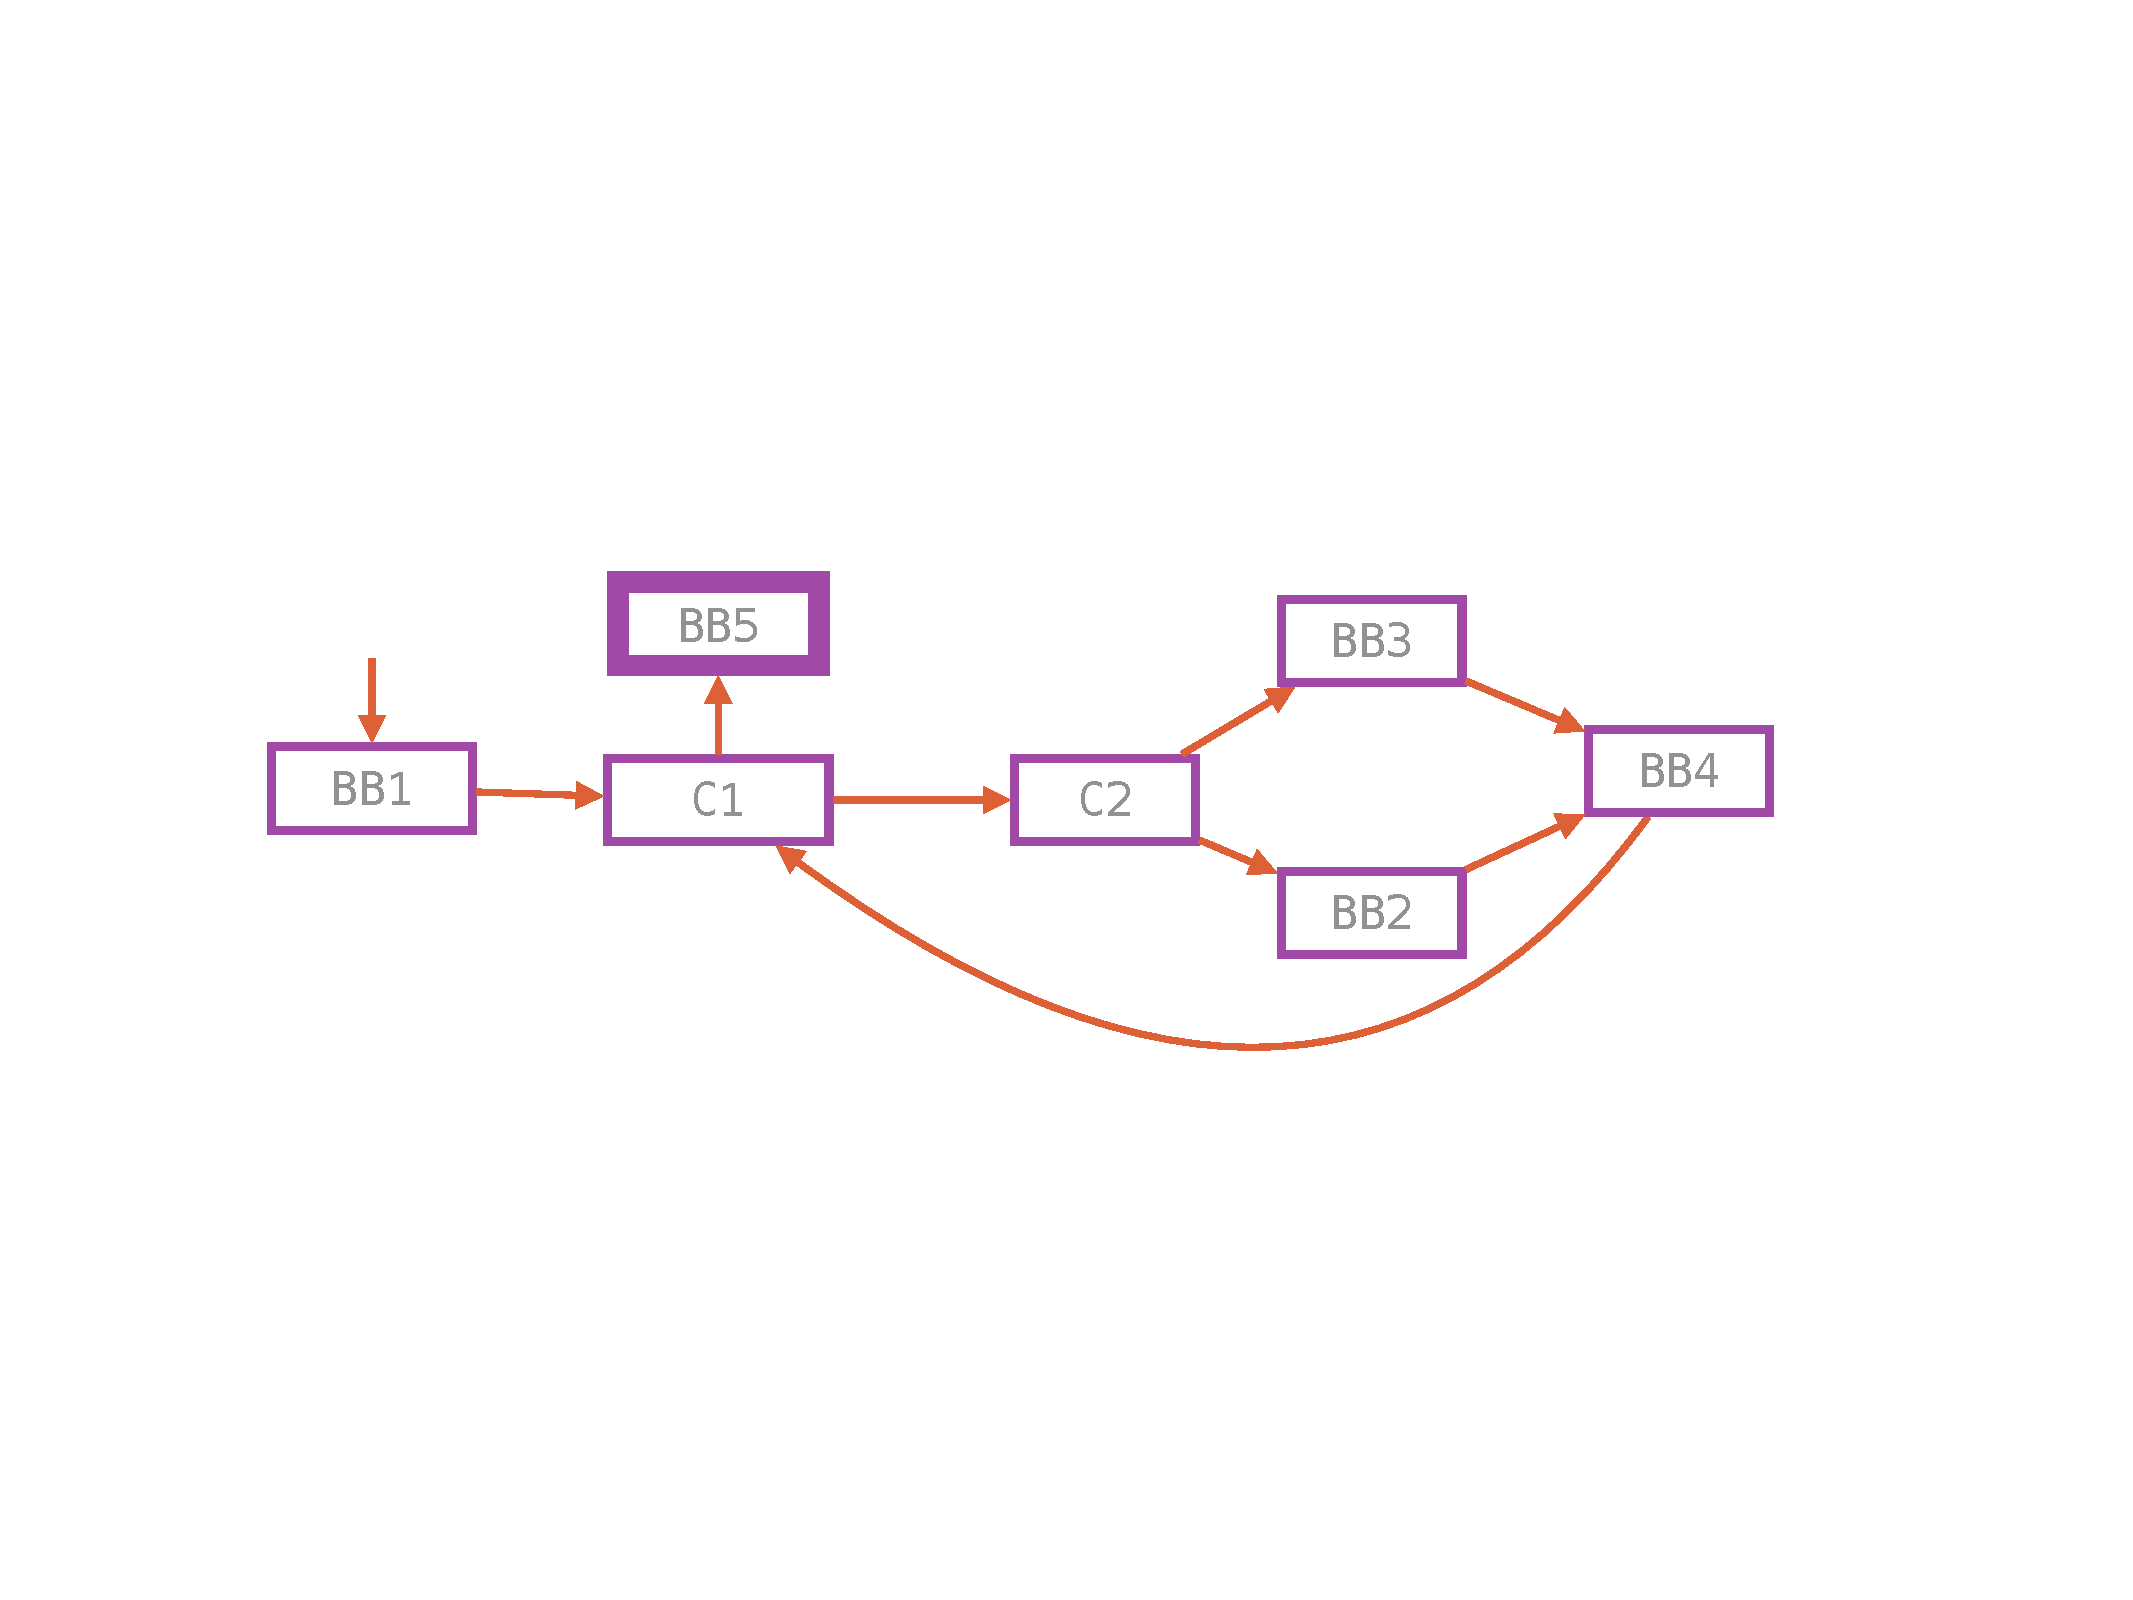
\includegraphics[width=.5\linewidth]{figures/midterm-cfg-1.pdf}
%     \end{center}
%   \end{figure}

%   \vspace{-1cm}
%   Please use the format [X, Y, Z] when writing paths. %
% \begin{parts}
% \part[3] If possible, provide 2 valid test paths through this
%   program. If this is not possible, explain why. %
%   \answerspace{11} %
%   \begin{solution}
%     E.g.\ [1, 3, 4, 5] and [1, 2, 4, 5]. A test path must begin at the
%     initial node and end at a terminal node.
%   \end{solution}

% \part[3] If possible, list 3 simple paths that (a) are not prime paths
%   and (b) start on node 2. If this is not possible, explain why. %
%   \answerspace{11} %
%   \begin{solution}
%     Any three of: [2], [2, 4], [2, 4, 5], [2, 4, 1].
%   \end{solution}

% \newpage
% \begin{center}
%   [PAGE DELIBERATELY LEFT BLANK]
% \end{center}
% \newpage

% \part[5] If possible, list four prime paths that start on node 4. If
%   this is not possible, explain why. %
%   \answerspace{11} %
%   \begin{solution}
%     Not possible --- there are only two: [4, 1, 2, 4] and
%     [4, 1, 3, 4]. Six simple paths start at node 4, but the other four
%     are proper subpaths of these two, so they are not prime.
%   \end{solution}

% \part[4] Write an example of a syntactically valid Java function that
%   generates this control-flow graph. If this is not possible, explain
%   why. %
%   \answerspace{25} %
%   \begin{solution}
%     %% FILL IN once the figure's node labels are settled.
%   \end{solution}

% \end{parts}

% \newpage
% \begin{center}
%   [PAGE DELIBERATELY LEFT BLANK]
% \end{center}
% \newpage

% ========================================================
% Q5: coverage feasibility.  [from midterm.tex Q2]
% ========================================================

\question Consider the following Python program:
  \vspace{-.3cm}
  \begin{minted}{python}
# Computes the square of x
def square(x: int) -> int:
  y = abs(x)
  z = 0
  while 0 < y:
    if z <= x * x:
      z += abs(x)
    y = y - 1
  return z
\end{minted}

\begin{parts}

\part[4] Is it feasible to devise a set of test cases that achieve
  100\% \textbf{node coverage} for \Code{square}? If your answer is
  yes, provide a minimal set of test cases that do so. If your answer
  is no, (a) provide a \emph{simple} change to \Code{square} so that it
  becomes possible, and (b) provide a simple, minimal test case set
  that then satisfies node coverage. Write your test cases in the
  form \Code{square(...)}. %
  \answerspace{14} %
  \begin{solution}
    Yes. The \Code{if} has no \Code{else}, so every node lies on the
    path taken when the condition is true. A single test, e.g.\
    \Code{square(1)}, visits every node.
  \end{solution}

\part[4] Is it feasible to devise a set of test cases that achieve
  100\% \textbf{edge coverage} for \Code{square}? If your answer is
  yes, provide a minimal set of test cases that do so. If your answer
  is no, (a) provide a \emph{simple} change to \Code{square} so that it
  becomes possible, and (b) provide a simple, minimal test case set
  that then satisfies edge coverage. Write your test cases in the
  form \Code{square(...)}. %
  \answerspace{14} %
  \begin{solution}
    No. Edge coverage requires the \emph{false} branch of
    \Code{if z <= x * x:}, and that branch is infeasible: on the $k$-th
    iteration \Code{z} holds $(k-1)\cdot|x|$, the loop runs $|x|$
    iterations, and $(k-1)\cdot|x| \leq x^2$ for every such $k$. So
    the condition is true on every evaluation, for every input.

    A simple change: replace the guard with something that can fail,
    e.g.\ \Code{if z <= x:}. Then \Code{square(3)} takes both
    branches and satisfies edge coverage.
  \end{solution}

\newpage
\begin{center}
  [PAGE DELIBERATELY LEFT BLANK]
\end{center}
\newpage

\part[4] Is it feasible for a set of test cases to achieve
  \textbf{complete path coverage} for \Code{square}? If your answer is
  yes, provide a minimal set of test cases that do so. If your answer
  is no, explain why not. Write your test cases in the form
  \Code{square(...)}. %
  \answerspace{15} %
  \begin{solution}
    No. The loop runs $|x|$ times, so for every $n$ there is a test
    path through the loop of length $n$ --- the set of test paths is
    infinite, and no finite test set can tour them all.
  \end{solution}

\end{parts}

\newpage
\begin{center}
  [PAGE DELIBERATELY LEFT BLANK]
\end{center}
\newpage

% Dropping to keep exam length reasonable
% ========================================================
% Q6: RIPR on a faulty program.  [from midterm.tex Q3]
% ========================================================

% \question Consider the following faulty Java program:
%   \vspace{-.3cm}
%   \begin{minted}{java}
% // Sums all elements in a non-null list, assuming no integer under/overflow
% public static int sum(List<Integer> numbers) {
%   int total = 0;
%   for (int i = 0; i < numbers.size() - 1; i++) {
%     total += numbers.get(i);
%   }
%   return total;
% }
% \end{minted}

% \begin{parts}
% \part[3] State the location(s) of the program fault and explain how you
%   would rewrite the line(s) to fix the fault. Your fixes should be as
%   simple as possible --- do not completely rewrite the function! %
%   \answerspace{16} %
%   \begin{solution}
%     Line 4. The loop bound \Code{numbers.size() - 1} stops one element
%     early, so the last element is never added. Replace it with
%     \Code{numbers.size()}.
%   \end{solution}

% \part[3] If possible, provide an example of a test input that does not
%   cause the fault to execute. If this is not possible, explain why. %
%   \answerspace{16} %
%   \begin{solution}
%     Not possible. The faulty expression is the loop guard, which is
%     evaluated on every call --- including when the list is empty.
%     There is no branch that can skip it.
%   \end{solution}

% \newpage
% \begin{center}
%   [PAGE DELIBERATELY LEFT BLANK]
% \end{center}
% \newpage

% \part[3] If possible, provide an example of a test input that causes
%   the fault to execute and triggers an error state, but does not result
%   in a failure. If this is not possible, explain why. %
%   \answerspace{20} %
%   \begin{solution}
%     Possible. E.g.\ \Code{[3, 0]}: the loop exits one iteration early,
%     so the program's state differs from that of the correct version
%     (an error state), but the skipped element is \Code{0}, so the
%     returned value 3 is still correct and no failure is observed.

%     Any list whose last element is \Code{0} works. Note that an empty
%     list does \emph{not} work: the correct and faulty versions behave
%     identically, so no error state arises.
%   \end{solution}

% \end{parts}

% \newpage
% \begin{center}
%   [PAGE DELIBERATELY LEFT BLANK]
% \end{center}
% \newpage

% ========================================================
% Q7: data-flow.  [from midterm.tex Q4, trimmed to 2 variables,
% converted to python]
% ========================================================

\question Consider the following Python implementation of a simple
  guessing game and its corresponding CFG, partially annotated with
  def-use information:\footnote{The CFG abbreviates the variables
    \mintinline{python}{secret_number} and
    \mintinline{python}{attempts} as \mintinline{python}{sn} and
    \mintinline{python}{att}, respectively. } \\
  \begin{tabular}{c|c}
    \begin{minipage}{.52\linewidth}
  \begin{minted}{python}
def guessing_game():
  secret_number = 42
  attempts = 1
  print("Try to guess the secret number.")
  while True:
    if attempts == 5:
      hint = secret_number % 10
      print("Hint: the last digit is", hint)
    guess = int(input("Enter your guess: "))
    if guess < secret_number:
      print("Too low!")
      attempts = attempts + 1
    elif guess > secret_number:
      print("Too high!")
      attempts = attempts + 1
    else:
      break
  print("Correct in only", attempts, "tries!")
\end{minted}
    \end{minipage}
    &
      \begin{minipage}{.44\linewidth}
        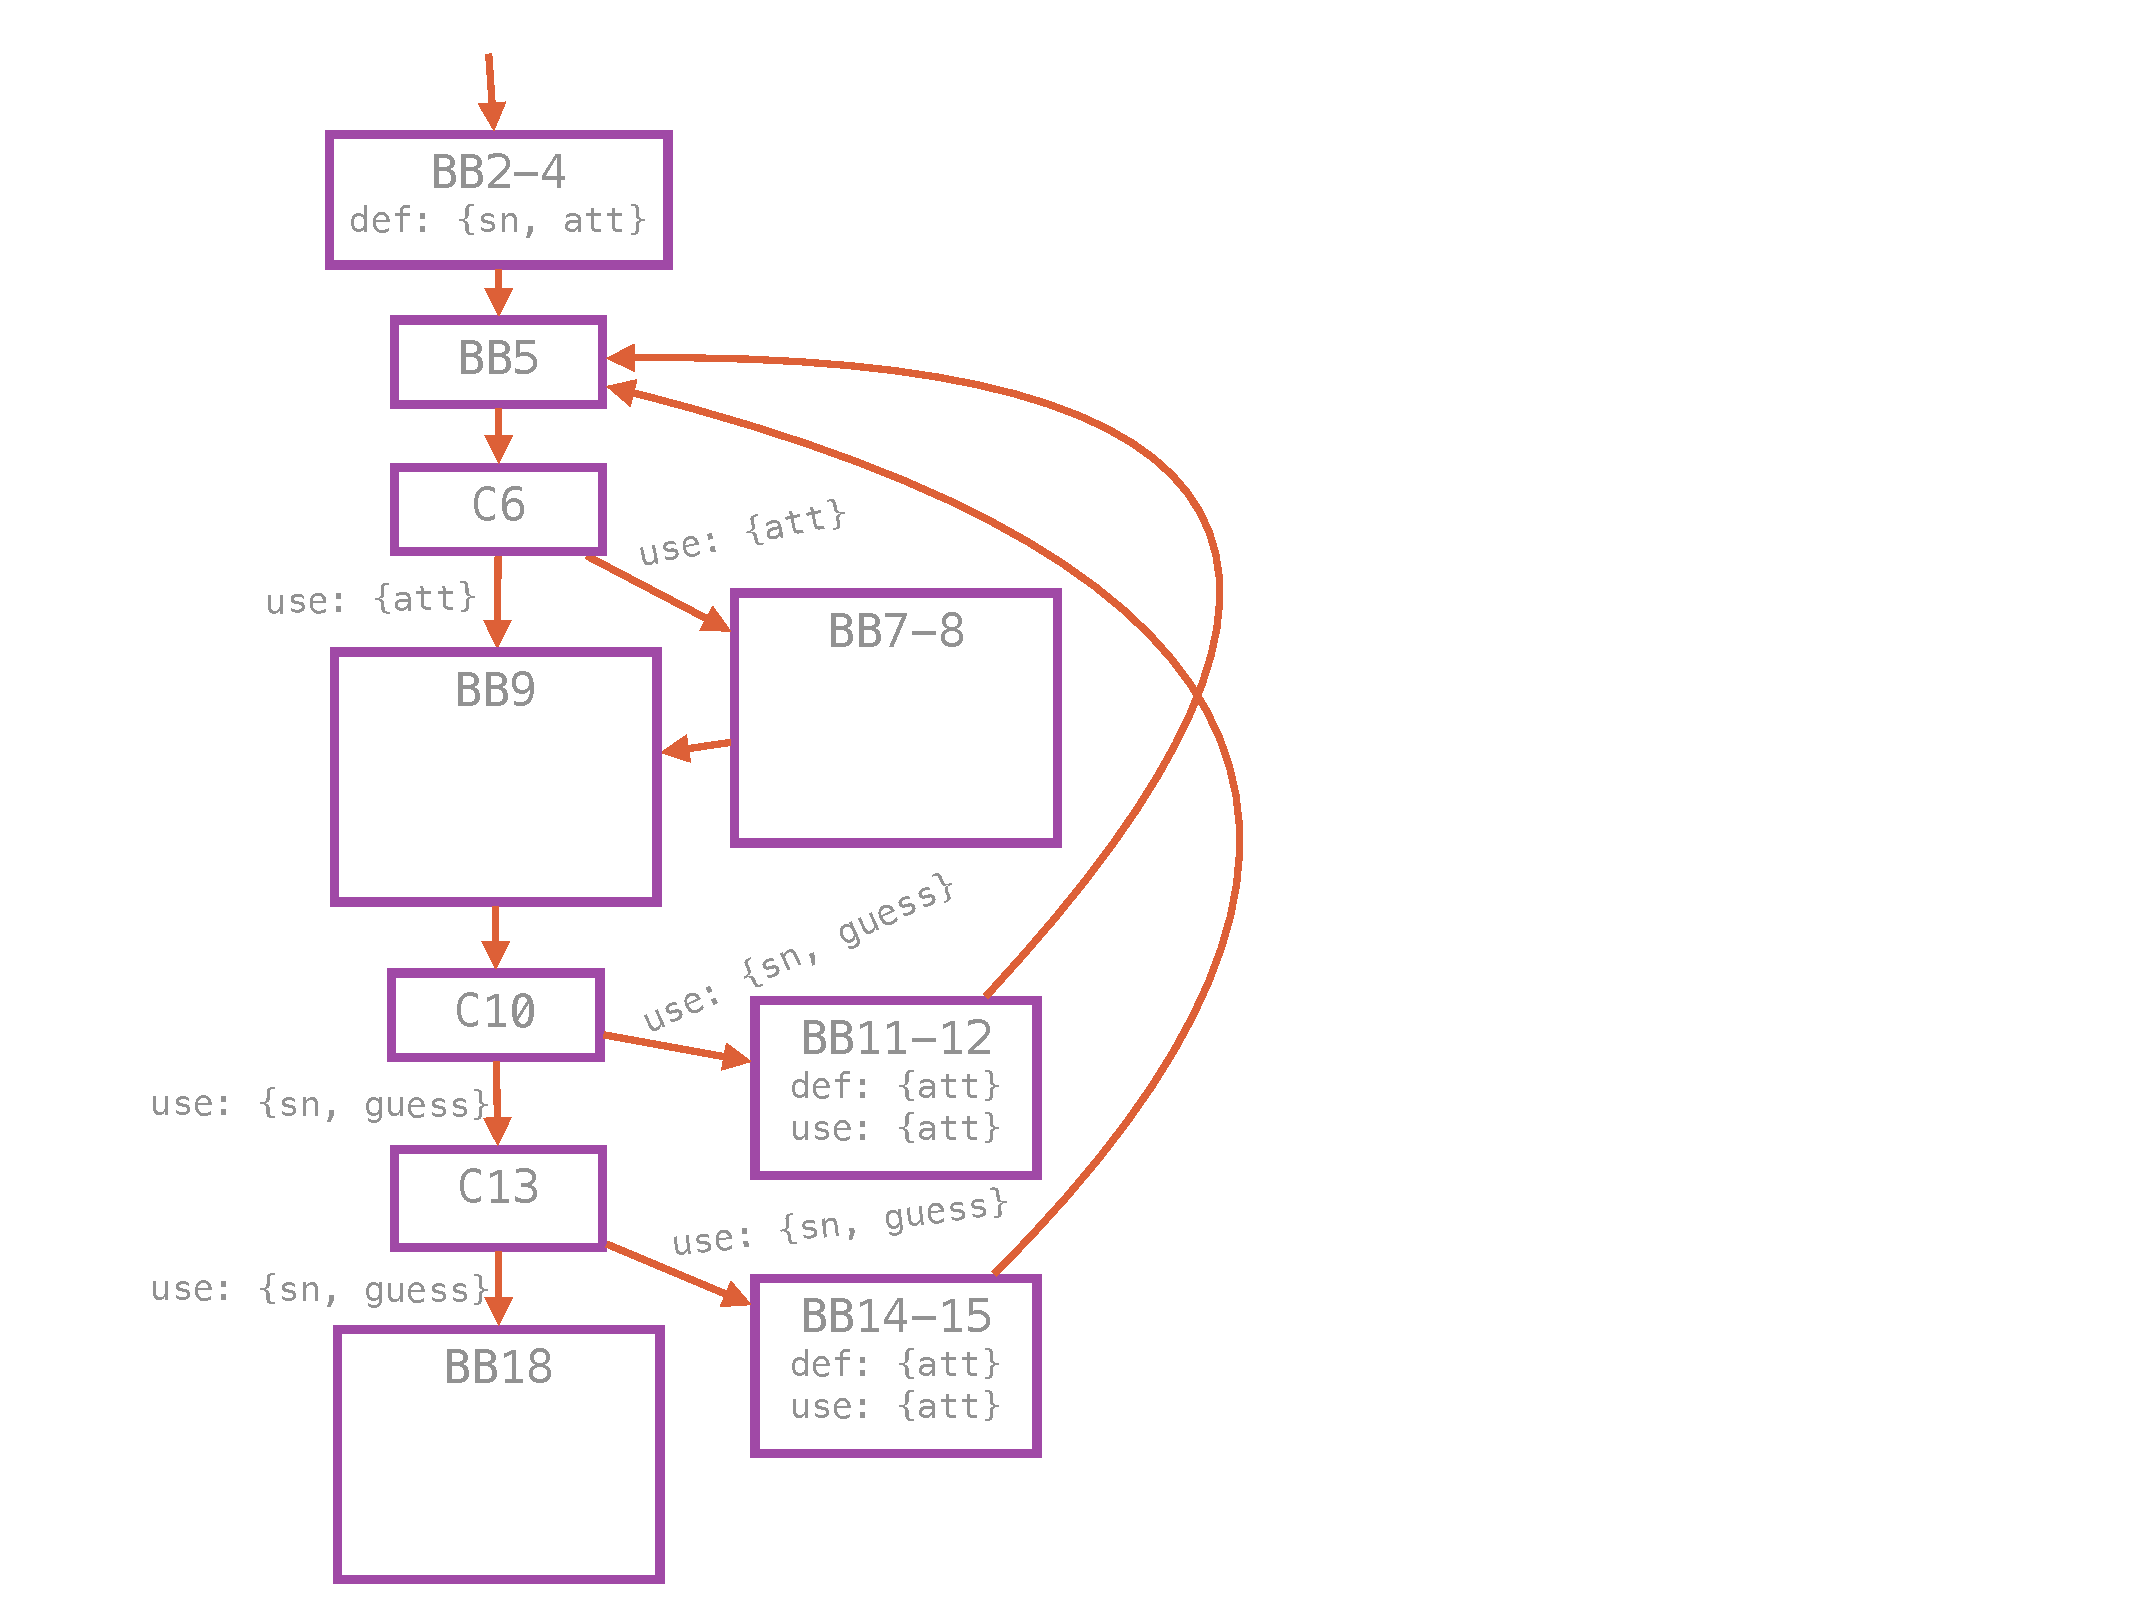
\includegraphics[width=.95\linewidth]{figures/du-cfg-1.pdf}
      \end{minipage}
  \end{tabular}

  \begin{parts}
  \part[2] Annotate the nodes of the above CFG with any missing
    def-use information. Feel free to abbreviate the variables
    \mintinline{python}{secret_number} as \mintinline{python}{sn} and
    \mintinline{python}{attempts} as \mintinline{python}{att}. %

    \phantom{foo} \\

  \part[2] List all the DU-pairs for the variable \Code{secret_number}.
  Please use the format (Line \#X, Line \#Y). %
  \answerspace{18} %
  \begin{solution}
    \Code{secret_number} is defined once, on line 2, and never
    redefined, so every use forms a pair:
    (2, 7), (2, 10), (2, 13).
  \end{solution}

\newpage
\begin{center}
  [PAGE DELIBERATELY LEFT BLANK]
\end{center}
\newpage

\part[5] List all the DU-pairs for the variable \Code{attempts}. Please
  use the format (Line \#X, Line \#Y). %
  \answerspace{26} %
  \begin{solution}
    Definitions are on lines 3, 12 and 15; uses are on lines 6, 12, 15
    and 18.%  (note that \Code{attempts += 1} both uses and defines
    % \Code{attempts})
     Every definition reaches every use along some
    def-clear path, giving twelve pairs:

    (3, 6), (3, 12), (3, 15), (3, 18), \\
    (12, 6), (12, 12), (12, 15), (12, 18), \\
    (15, 6), (15, 12), (15, 15), (15, 18).

    The eight pairs defined on lines 12 and 15 all require a test that
    enters the loop body at least twice.
  \end{solution}
\end{parts}

\newpage
\begin{center}
  [PAGE DELIBERATELY LEFT BLANK]
\end{center}
\newpage

% ========================================================
% Q8: logic coverage.  [from final.tex Q5]
% ========================================================

\question Consider the following Python program:
  \vspace{-.3cm}
  \begin{minted}{python}
def foo(x: int, y: str, z: int) -> int:
    out = 0
    if z > 0 or (x < -10 and y == "y"):
        out = 1
    else:
        out = 2
    return out
\end{minted}
\begin{parts}

\part[3] Give a minimal test set that achieves 100\% \textbf{predicate
    coverage} for \Code{foo}. If this is not possible, explain why in
  2--3 sentences. Write your test cases in the form
  \Code{foo(..., ..., ...)}.%
  \answerspace{16} %
  \begin{solution}
    Two tests suffice: one making the predicate true, e.g.\
    \ACC{0}{"0"}{1}, and one making it false, e.g.\ \ACC{0}{"0"}{-1}.
  \end{solution}

\part[3] Give a test set that achieves 100\% \textbf{clause coverage}
  but \textit{not} 100\% predicate coverage for \Code{foo}. If this is
  not possible, explain why in 2--3 sentences. Write your test cases
  in the form \Code{foo(..., ..., ...)} %
  \answerspace{16} %
  \begin{solution}
    \ACC{0}{"0"}{1} and \ACC{-20}{"y"}{0}. Each clause takes both
    values across the two tests, but the predicate is true in both.
  \end{solution}

\newpage
\begin{center}
  [PAGE DELIBERATELY LEFT BLANK]
\end{center}
\newpage

\part[5] Give a test set that achieves 100\% \textbf{General Active
    Clause Coverage} (GACC) but \textit{not} 100\% predicate coverage
  for \Code{foo}. If this is not possible, explain why in 2--3
  sentences. Write your test cases in the form \Code{foo(..., ...,
    ...)} %
  \answerspace{20} %
  \begin{solution}
    Not possible. Whenever a clause of this predicate determines it,
    the predicate's value is forced to equal that clause's value ---
    for instance, \Code{x < -10} determines the predicate only when
    \Code{z > 0} is false and \Code{y == "y"} is true, and under that
    assignment the predicate is true exactly when \Code{x < -10} is.
    The same holds for the other two clauses. GACC requires a pair of
    tests making some clause true and false while it determines the
    predicate, and any such pair therefore makes the predicate both
    true and false --- which is predicate coverage.
  \end{solution}
\end{parts}

\newpage
\begin{center}
  [PAGE DELIBERATELY LEFT BLANK]
\end{center}
\newpage

% ========================================================
%% Q9: mutation testing.  [NEW]
% ========================================================

\question Consider the following Python program, which calculates a
  score by awarding ten points per hit and assesses a five point
  penalty for more than three misses.  The score is never negative.
  \vspace{-.3cm}
  \begin{minted}{python}
def score(hits: int, misses: int) -> int:
  s = hits * 10
  if misses > 3:
    s = s - 5
  if s < 0:
    s = 0
  return s
\end{minted}
\begin{parts}

\part[3] Consider a mutant that replaces line 3 with \Code{if misses
    >= 3:}. Give a test case that \textbf{kills} this mutant, or
  explain in 2-3 sentences why you cannot. As before, write your test
  case in the form \Code{score(..., ...)}. %
  \answerspace{16} %
  \begin{solution}
    Any input with exactly three misses. E.g.\
    \Code{score(1, 3)}: the original returns 10, the mutant returns 5.
  \end{solution}

\part[3] Consider a different mutant that replaces line 5 with
  \Code{if s <= 0:}. Give a test case that \textbf{kills} this mutant, or
  explain in 2-3 sentences why you cannot. As before, write your test
  case in the form \Code{score(..., ...)}. %
  \answerspace{16} %
  \begin{solution}
    No such test exists: this is an \textbf{equivalent mutant}. The
    two versions differ only when \Code{s} is exactly 0, and in that
    case the mutant executes \Code{s = 0}, which changes
    nothing. Since no input distinguishes them, this mutant can never
    be killed, and a kill rate of 100\% is unachievable for this
    program.
  \end{solution}

\newpage
\begin{center}
  [PAGE DELIBERATELY LEFT BLANK]
\end{center}
\newpage

\part[2] Using the RIPR model, explain in 2--3 sentences why a test
  case that \emph{executes} a mutated statement may nonetheless fail to
  kill the mutant. %
  \answerspace{18} %
  \begin{solution}
    Executing the mutated statement establishes only \emph{reachability}.
    The mutant is killed only if the mutation also causes the program
    state to differ (\emph{infection}) and that difference reaches the
    output (\emph{propagation}), where it must be observable in the
    result the test checks. A test can reach a mutated line and still
    compute the same value, or compute a different intermediate value
    that is later overwritten or masked.
  \end{solution}

\end{parts}

% \newpage
% \begin{center}
%   [PAGE DELIBERATELY LEFT BLANK]
% \end{center}
% \newpage

\if 0 %%%%%%%%%%%%%%%%%%%%%%%%%%%%%%%%%%%%%%%%%
	\question[10]
	\answerspace{30}
	\begin{solution}
        \end{solution}
\fi %%%%%%%%%%%%%%%%%%%%%%%%%%%%%%%%%%%%%%%%%

	\newpage
	\begin{center}
		[EMPTY PAGE 1 -- Use as overflow to complete your
                answers ]
	\end{center}

	\newpage
	\begin{center}
		[EMPTY PAGE 2 -- Use as overflow to complete your
                answers ]
              \end{center}

\end{questions}

\end{document}
